\chapter{Aritmética de ideales}

La idea de Richard Dedekind consistía en remplazar las operaciones aritméticas
con elementos $\alpha \in R$ por las operaciones con ideales $I\subseteq R$.
Los anillos de números donde este programa funciona sin obstáculos se conocen
como los \textbf{anillos de Dedekind}. Los vamos a definir en este capítulo.

Una gran parte del material de abajo (ideales primos y maximales, localización,
dominios de valuación discreta, etc.) se encuentra en los libros de texto de
álgebra conmutativa. Recomiendo consultar \cite{Atiyah-Macdonald} y
\cite{Reid-UCA}.

\begin{figure}
  \begin{center}
    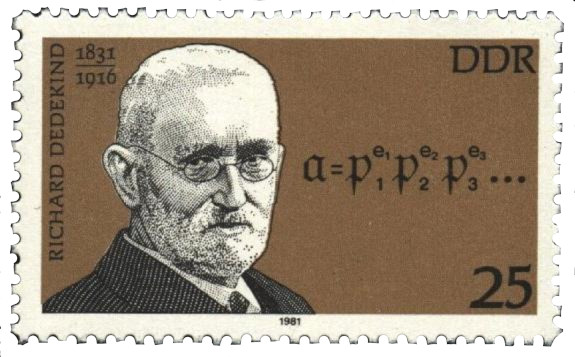
\includegraphics[width=7cm]{pic/Dedekind_stamp.jpg}
  \end{center}

  \caption{Estampilla de la República Democrática Alemana dedicada a Dedekind}
\end{figure}

\pdfbookmark{Clase 5 (24/08/20)}{clase-5}
\section{Operaciones con ideales}
\marginpar{\small Clase 5 \\ 24/08/20}


Sea $R$ un anillo conmutativo. Ya hemos hablado de ideales principales en
el primer capítulo. En general, el ideal generado por elementos
$\alpha_1,\ldots,\alpha_n \in R$ viene dado por
\[ (\alpha_1,\ldots,\alpha_n) =
   \{ c_1 \alpha_1 + \cdots + c_n \alpha_n \mid c_1,\ldots,c_n \in R \}. \]
Los ideales de esta forma se llaman \textbf{finitamente generados}.

\begin{definicion}
  Para los ideales $I, J \subseteq R$ podemos considerar las siguientes
  operaciones.

  \begin{itemize}
  \item La \textbf{suma}
    $$I + J = \{ \alpha + \beta \mid \alpha \in I, \, \beta \in J \}$$
    es el ideal generado por los elementos de $I$ y $J$; en otras palabras,
    el ideal más pequeño que contiene a $I$ e $J$.

    En términos de generadores,
    \[ (\alpha_1,\ldots,\alpha_m) + (\beta_1,\ldots,\beta_n) =
       (\alpha_1,\ldots,\alpha_m,\beta_1,\ldots,\beta_n). \]

  \item El \textbf{producto}
    \[ IJ = \Bigl\{ \sum_{1 \le i \le n} \alpha_i \beta_i \Bigm|
                    n \ge 0, \, \alpha_i \in I, \, \beta_i \in J  \Bigl\} \]
    es el ideal generado por los productos $\alpha\beta$, donde $\alpha \in I$, $\beta \in J$.
    En términos de generadores,
    \[ (\alpha_1,\ldots,\alpha_m) \cdot (\beta_1,\ldots,\beta_n) =
       (\alpha_i \beta_j)_{\substack{1 \le i \le m \\ 1 \le j \le n}}. \]

    Notamos que se cumple $IJ \subseteq I\cap J$.
  \end{itemize}
\end{definicion}

Es fácil verificar que $+$ y $\cdot$ son operaciones asociativas y conmutativas
sobre ideales. Tenemos
$$I + (0) = I, ~ I + R = R, ~ I \cdot (0) = (0), ~ I\cdot R = I.$$
Además, se cumple la distributividad
$$(I + J) H = IH + JH$$
---dejo al lector verificar la doble inclusión.

Ya que hemos definido productos, podemos definir las potencias de la manera
habitual:
\[ I^0 = R, \quad
I^1 = I, \quad
I^2 = I\cdot I, \quad
I^3 = I\cdot I\cdot I, \quad
\ldots \]
Estas nos dan una cadena descendiente
$$R \supseteq I \supseteq I^2 \supseteq I^3 \supseteq \cdots$$

\begin{comentario}
  Cuidado: los elementos de $I^n$ no son productos de $n$ elementos de $I$
  (y mucho menos potencias $\alpha^n$ para $\alpha \in I$), sino \emph{sumas}
  de productos
  $$\sum_{i_1,\ldots,i_n} \alpha_{i_1} \cdots \alpha_{i_n}.$$
  Por ejemplo, en el anillo de polinomios $\ZZ [x]$, consideremos el ideal
  $I = (p,x)$. Entonces $p^2 + x^2 \in I$, pero este elemento no es de la forma
  $fg$ con $f,g \in I$.
\end{comentario}

Notamos que si $J = IH$ para algún $H$, entonces se tiene $J \subseteq H$.
Además, para los ideales principales se cumple
$$\alpha \mid \beta \iff (\alpha) \supseteq (\beta).$$
Esto justifica de alguna manera la siguiente definición.

\begin{definicion}
  Se dice que $I$ divide a $J$ (notación $I \mid J$) si $J \subseteq I$.
\end{definicion}

Sin embargo, hay que tener cuidado: en general no es cierto que $J \subseteq I$
siempre implica que $J = IH$ para algún ideal $H$. Vamos a ver un ejemplo
particular un poco más adelante.

\begin{definicion}
  Se dice que dos ideales $I,J \subseteq R$ son \textbf{coprimos} si
  $I + J = R$.
\end{definicion}

\begin{comentario}
  La motivación detrás del término ``coprimo'' es la siguiente:
  en un dominio de ideales principales (!) se tiene
  \[ (\alpha) + (\beta) = (\alpha,\beta) = (\gamma), \quad
     \text{donde }\gamma = \gcd (\alpha,\beta). \]
  Entonces, $\gcd (\alpha,\beta) = 1$ implica que $(\alpha)+(\beta) = R$.
 
  En general (si $R$ no es un dominio de ideales principales), esto no es
  cierto. Por ejemplo, en el anillo de polinomios $k[x,y]$ se tiene $\gcd (x,y)
  = 1$: los polinomios $x$ e $y$ claramente no tienen divisor en común (excepto
  constantes $c\ne 0$). Por otra parte, $(x,y) \ne k [x,y]$; de hecho,
  $k [x,y]/(x,y) \cong k$.

  Otro ejemplo, más relacionado con lo que estamos estudiando: en el anillo
  $\ZZ [\sqrt{-5}]$ consideremos el ideal $(2, 1 + \sqrt{-5})$. Sus dos
  generadores $2$ y $1 + \sqrt{-5}$ son elementos irreducibles no asociados
  entre sí, y por ende no tienen divisor en común. Sin embargo, no es difícil
  verificar que el ideal en cuestión es propio (y de hecho no es principal).
\end{comentario}

Ahora bien, ¿para qué sirven los ideales y operaciones aritméticas con ellos?
En el capítulo anterior hemos usado en algunas ocasiones que en un dominio
de factorización única, si $\gcd (\alpha,\beta) = 1$
y $\alpha\beta = \gamma^n$, entonces $\alpha$ y $\beta$ (salvo un múltiplo
invertible) son $n$-ésimas potencias: $\alpha \sim \alpha'^n$ y
$\beta \sim \beta'^n$.

Si no hay factorización única, esta propiedad falla.

\begin{ejemplo}
  Ya hemos notado que en el anillo $\ZZ [\sqrt{-5}]$ se tiene
  $$(2 + 3\sqrt{-5})\,(2 - 3\sqrt{-5}) = 7^2,$$
  donde $2 \pm 3\sqrt{-5}$ no es un cuadrado. Para corregir este defecto,
  se puede pasar a los ideales. Pongamos
  \[ I = (2 + 3\sqrt{-5}), \quad J = (2 - 3\sqrt{-5}), \quad H = (7). \]
  Tenemos
  $$I + J = R, \quad I J = H^2.$$
  Ahora
  $$(I + H)^2 = I^2 + I H + H^2 = I\,(I + H + J) = I,$$
  usando que $I + J = R$. De manera simétrica, $(J + H)^2 = J$. Entonces, aunque
  los números $2 \pm 3\sqrt{-5}$ no son cuadrados, los ideales principales
  generados por ellos sí lo son:
  $$(7, 2 \pm 3\sqrt{-5})^2 = (2 \pm 3\sqrt{-5}).$$
  El único detalle es que el ideal $(7, 2 \pm 3\sqrt{-5})$ no es principal;
  de manera contraria, tendríamos $2 \pm 3\sqrt{-5} = \pm\alpha^2$ para algún
  $\alpha$, pero no es el caso.
\end{ejemplo}

El truco de arriba funciona en general.

\begin{proposicion}
  \label{prop:producto-de-ideales-coprimos}
  Sean $I, J$ dos ideales tales que $I + J = R$ e $I J = H^n$.
  Entonces, $(I + H)^n = I$.

  \begin{proof}
    Primero una observación: si $I + J = R$, entonces $I^m + J = R$ para todo
    $m$. En efecto,
    \[ R = (I + J)^m =
       I^m + \underbrace{I^{m-1} J + \cdots + I J^{m-1} + J^m}_{\subseteq J}
       \subseteq I^m + J. \]

    Ahora
    \begin{align*}
      (I + H)^n & = I^n + I^{n-1} H + \cdots + I H^{n-1} + H^n \\
                & = I^n + I^{n-1} H + \cdots + I H^{n-1} + I J \\
                & = I\,(I^{n-1} + I^{n-2} H + \cdots + H^{n-1} + J) \\
                & = I,
    \end{align*}
    usando que $I^{n-1} + J = R$.
    \end{proof}
\end{proposicion}

Para terminar con la aritmética básica de ideales, revisemos el teorema chino
del resto. En un dominio de ideales principales este nos dice que
si $\gcd (\alpha,\beta) = 1$, entonces
$$R/(\alpha\beta) \cong R/(\alpha) \times R/(\beta).$$
En un anillo general, hay que considerar ideales coprimos. Primero hagamos
una pequeña observación

\begin{lema}
  Si $I + J = R$, entonces $I \cap J = IJ$.

  \begin{proof}
    Tenemos $IJ \subseteq I\cap J$ en cualquier caso. Ahora si $I + J = R$,
    escribamos $1 = \alpha + \beta$ para $\alpha \in I$, $\beta \in J$.
    Para todo $\gamma \in I \cap J$ se tiene entonces
    $$\gamma = \gamma\,(\alpha + \beta) = \gamma \alpha + \gamma \beta \in IJ.$$
    Esto demuestra la otra inclusión.
  \end{proof}
\end{lema}

Ahora el teorema chino del resto para anillos conmutativos es el siguiente
resultado.

\begin{teorema}[chino del resto]
  Sean $I, J \subseteq R$ ideales tales que $I + J = R$. Luego, hay un
  isomorfismo natural
  \begin{align*}
    R/(IJ) & \xrightarrow{\cong} R/I \times R/J,\\
    \alpha + IJ & \mapsto (\alpha + I, \alpha + J).
  \end{align*}

  \begin{proof}
    Consideremos el homomorfismo
    \[ \phi\colon R \to R/I \times R/J, \quad
       x \mapsto (x+I,x+J). \]
    Vamos a ver que es sobreyectivo y su núcleo es igual a $IJ$.

    Para ver la sobreyectividad, necesitamos probar que para cualesquiera
    $\alpha,\beta\in R$ existe $x\in I$ tal que
    $$x \equiv \alpha \pmod{I}, \quad x \equiv \beta \pmod{J}.$$
    De nuevo, dado que $I + J = R$, escribamos $a + b = 1$ para $a \in I$, $b
    \in J$. Notamos que
    \[ a \equiv 0 \pmod{I}, \quad
       a \equiv 1 \pmod{J}, \quad
       b \equiv 1 \pmod{I}, \quad
       b \equiv 0 \pmod{J}. \]
    Se ve que funcionará el elemento
    $$x = b \alpha + a \beta.$$

    En fin, está claro que $\ker \phi = I \cap J$, y por el lema anterior
    $I \cap J = IJ$.
  \end{proof}
\end{teorema}

\begin{comentario}
  La condición $I + J = R$ es necesaria para la prueba. Por ejemplo, si
  $I = J = 2\ZZ$, entonces $\ZZ/4\ZZ \not\cong \ZZ/2\ZZ \times \ZZ/2\ZZ$.
\end{comentario}

De manera similar, se puede probar que para una familia de ideales
$I_1,\ldots,I_n$ tales que $I_i + I_j = R$ para $i\ne j$, se tiene un isomorfismo
natural
$$R/(I_1\cdots I_n) \cong R/I_1 \times \cdots \times R/I_n$$
(he tomado $n = 2$ en la prueba se arriba solo para simplificar la notación).

\begin{ejemplo}
  Para un primo racional $p \equiv 1 \pmod{4}$ se tiene
  $p = \pi\,\overline{\pi}$ en $\ZZ[i]$. Ya que se trata de un dominio
  de ideales principales, se tiene
  $$(\pi) + (\overline{\pi}) = (\gcd (\pi, \overline{\pi})) = \ZZ[i],$$
  así que por el teorema chino del resto
  \[ \ZZ[i]/(p) \cong \ZZ[i]/(\pi) \times \ZZ[i]/(\overline{\pi})
                \cong \FF_p\times \FF_p. \]
  Otro modo de ver qué está pasando: tenemos
  $$\ZZ[i] \cong \ZZ[x]/(x^2+1), \quad \ZZ[i]/(p) \cong \FF_p [x]/(x^2+1).$$
  Ahora $x^2 + 1$ es irreducible o reducible en $\FF_p [x]$ dependiendo del
  símbolo de Legendre $\legendre{-1}{p} = \pm 1$. Cuando es reducible módulo $p$
  impar, salen dos diferentes factores lineales $x \pm a$, donde $a^2 \equiv -1
  \pmod{p}$.
\end{ejemplo}

%%%%%%%%%%%%%%%%%%%%%%%%%%%%%%%%%%%%%%%%%%%%%%%%%%%%%%%%%%%%%%%%%%%%%%%%%%%%%%%%

\section{Ideales primos y maximales}

El concepto que remplaza la noción de elemento primo es el de \emph{ideal} primo.

\begin{definicion}
  Se dice que un ideal $\mathfrak{p} \subset R$ es \textbf{primo} si este cumple
  una de las siguientes propiedades equivalentes:\footnote{Ejercicio:
    a)$\iff$a${}'$)$\iff$b).}
  \begin{enumerate}
  \item[a)] $\mathfrak{p} \ne R$ y si $\alpha\beta \in \mathfrak{p}$, entonces
    $\alpha \in \mathfrak{p}$ o $\beta \in \mathfrak{p}$;

  \item[a${}'$)] $\mathfrak{p} \ne R$ y si $IJ \subseteq \mathfrak{p}$, entonces
    $I \subseteq \mathfrak{p}$ o $J \subseteq \mathfrak{p}$;
  
  \item[b)] el anillo cociente $R/\mathfrak{p}$ es un dominio.
  \end{enumerate}

  El conjunto de los ideales primos en $R$ se llama el \textbf{espectro}
  de $R$ y se denota por
  $$\Spec R = \{ \mathfrak{p} \subset R \mid \text{ ideal primo} \}.$$

  Se dice que un ideal $\mathfrak{m} \subset R$ es \textbf{maximal} si este
  cumple una de las siguientes propiedades equivalentes:\footnote{Ejercicio:
    a)$\iff$b).}
  \begin{enumerate}
  \item[a)] $\mathfrak{m} \ne R$ y si $\mathfrak{m} \subseteq I \subseteq R$,
    entonces $I = \mathfrak{m}$ o $I = R$;

  \item[b)] el anillo cociente $R/\mathfrak{m}$ es un campo.
  \end{enumerate}
\end{definicion}
(Por la definición, el anillo nulo $R = 0$ no se considera como un dominio,
mucho menos como un campo.)

\begin{proposicion}
  Todo ideal maximal es primo.

  \begin{proof}
    Está claro de la caracterización b).
  \end{proof}
\end{proposicion}

\begin{ejemplo}
  Si $R$ es un dominio de ideales principales, entonces los ideales primos son
  $$\Spec R = \{ (0) \} \cup \{ (\pi) \mid \pi \in R \text{ es primo} \}.$$
  Los ideales de la forma $(\pi)$ son maximales, dado que $R/(\pi)$ es un campo.

  Para verlo, notamos que el ideal principal $(\pi) \subset R$ es primo si y
  solamente si $\pi \in R$ es un elemento primo en el sentido del capítulo
  anterior. En particular,
  \[ \Spec \ZZ = \{ (0) \} \cup \{ (2), (3), (5), (7), (11), \ldots \}. \qedhere \]
\end{ejemplo}

\begin{ejemplo}
  En el anillo $\ZZ [\sqrt{-5}]$ consideremos los ideales
  \[ \mathfrak{p} = (7, 3 + \sqrt{-5}), \quad
     \overline{\mathfrak{p}} = (7, 3 - \sqrt{-5}). \]

  Los ideales en cuestión no son principales: primero, analizando las normas se
  ve que $7$ y $3 \pm \sqrt{-5}$ son elementos irreducibles no asociados
  (las unidades son $\pm 1$). Luego, si $\mathfrak{p} = (\gamma)$, podemos
  considerar las expresiones
  $$7 = \alpha\gamma, \quad 3 + \sqrt{-5} = \beta\gamma$$
  para llegar a una contradicción. Dejo al lector los detalles.

  Estos ideales son coprimos:
  \[ 1 = 7 - (3 + \sqrt{-5}) - (3 - \sqrt{-5})
     \in \mathfrak{p} + \overline{\mathfrak{p}}. \]
  Su producto viene dado por
  \begin{align*}
    \mathfrak{p}\overline{\mathfrak{p}} & = (7, 3+\sqrt{-5})\,(7, 3-\sqrt{-5}) \\
    & = \Bigl(7^2, 7\,(3 + \sqrt{-5}), 7\,(3 - \sqrt{-5}), 14\Bigr) \\
    & = (7)\,(\underbrace{7, 3 + \sqrt{-5}, 3 - \sqrt{-5}, 2}_{= R}) = (7).
  \end{align*}

  Los ideales $\mathfrak{p}$ y $\overline{\mathfrak{p}}$ son propios.
  Por ejemplo, si $\mathfrak{p} = \ZZ [\sqrt{-5}]$, entonces
  para algunos $a,b,c,d \in \ZZ$ se tiene
  \[ 1 = (a + b\sqrt{-5})\cdot 7 + (c + d\sqrt{-5})\cdot (3 + \sqrt{-5})
       = (7a + 3c + 3d) + (7b + c + d)\sqrt{-5}. \]
  De la ecuación $7b + c + d = 0$ podemos expresar $d = -7b-c$,
  y luego al sustituirlo en $1 = 7a + 3c + 3d$ nos queda
  $1 = 7a - 21b$, pero el número a la derecha es par.

  Otra manera más lista es notar que el grupo
  $$\Gal (\QQ (\sqrt{-5})/\QQ) = \{ 1, \sigma \},$$
  donde $\sigma\colon \sqrt{-5} \mapsto -\sqrt{-5}$, actúa sobre
  $\ZZ [\sqrt{-5}]$. Para un ideal $I \subset \ZZ [\sqrt{-5}]$
  el conjunto $\sigma (I)$ es también un ideal, y además, en términos
  de generadores,
  \[ \sigma (\alpha_1,\ldots,\alpha_n) =
     (\sigma (\alpha_1), \ldots, \sigma (\alpha_n)). \]

  En nuestro caso particular se tiene
  $\overline{\mathfrak{p}} = \sigma (\mathfrak{p})$. Ahora si
  $\mathfrak{p} = \ZZ [\sqrt{-5}]$, entonces también
  $\overline{\mathfrak{p}} = \ZZ [\sqrt{-5}]$, pero en este caso
  $\mathfrak{p}\,\overline{\mathfrak{p}} = \ZZ [\sqrt{-5}]$, lo que
  contradice nuestro cálculo de arriba.

  Los ideales $\mathfrak{p}$ y $\overline{\mathfrak{p}}$ son maximales.
  Para verlo, podemos considerar el homomorfismo sobreyectivo
  \[ \phi\colon \ZZ[\sqrt{-5}] \to \FF_7 [x]/(3 + x), \quad
     a + b\sqrt{-5} \mapsto a + b\overline{x}. \]
  (Note que $3^2 \equiv -5 \pmod{7}$.)
  Tenemos $\ker\phi = \mathfrak{p}$, y este ideal es maximal.
  De manera similar se define un homomorfismo sobreyectivo
  $$\overline{\phi}\colon \ZZ[\sqrt{-5}] \to \FF_7 [x]/(3 - x),$$
  donde $\ker\overline{\phi} = \overline{\mathfrak{p}}$.

  Notamos que en general, un homomorfismo $\phi\colon \ZZ [\sqrt{-5}] \to \FF_7$
  está definido por la imagen de $\sqrt{-5}$ que debe cumplir
  $\phi (\sqrt{-5})^2 = -5$ en $\FF_p$. Las únicas posibilidades son
  $\phi (\sqrt{-5}) = \pm 3$, así que hemos encontrado los únicos dos ideales
  maximales que cumplen $\ZZ [\sqrt{-5}]/\mathfrak{p} \cong \FF_7$.

  El teorema chino del resto nos da en este caso
  \[ \begin{tikzcd}
    \ZZ [\sqrt{-5}]/(7) \ar{d}{\cong} &[-3em] \cong &[-3em] \ZZ[\sqrt{-5}]/\mathfrak{p} \ar{d}{\cong} &[-3em] \times &[-3em] \ZZ[\sqrt{-5}]/\overline{\mathfrak{p}} \ar{d}{\cong} \\
    \FF_7 [x]/(x^2 + 5) & \cong & \FF_7 [x]/(3 + x) \ar{d}{\cong} & \times & \FF_7 [x] / (3 - x) \ar{d}{\cong} \\
     && \FF_7 & \times & \FF_7
  \end{tikzcd} \]
\end{ejemplo}

\begin{proposicion}
  Un homomorfismo de anillos $\phi\colon S\to R$ induce una aplicación natural
  entre los espectros
  $$\phi^{-1}\colon \Spec R\to \Spec S, \quad
    \mathfrak{p} \mapsto \phi^{-1} (\mathfrak{p}).$$

  \begin{proof}
    Verifique si $\mathfrak{p} \subset R$ es un ideal primo, entonces
    $\phi^{-1} (\mathfrak{p})$ es un ideal primo en $S$.
  \end{proof}
\end{proposicion}

\begin{ejemplo}
  La inclusión natural $\ZZ \hookrightarrow \ZZ [\sqrt{-5}]$ induce
  una aplicación $\Spec \ZZ [\sqrt{-5}] \to \Spec \ZZ$ dada por
  $\mathfrak{p} \mapsto \mathfrak{p} \cap \ZZ$. En el ejemplo de arriba,
  \[ (7, 3 \pm \sqrt{-5}) \cap \ZZ = 7\ZZ. \qedhere \]
\end{ejemplo}

También nos servirá la siguiente propiedad.

\begin{proposicion}
  Dado un ideal propio $I \subsetneq R$, existe un ideal maximal
  $\mathfrak{m} \subset R$ tal que $I \subseteq \mathfrak{m}$.

  \begin{proof}
    Esta es una aplicación típica del lema de Zorn.

    Sea $\mathcal{P}$ el conjunto de los ideales propios
    $I \subseteq J_\alpha \subsetneq R$ parcialmente ordenado respecto a la
    inclusión $J_\alpha \subseteq J_\beta$. Un elemento maximal en $\mathcal{P}$
    sería precisamente un ideal maximal en $R$ que contiene a $I$. Para deducir
    la existencia de un elemento maximal, tenemos que probar que toda cadena en
    $\mathcal{P}$ es acotada.

    Una cadena en $\mathcal{P}$ es una colección de ideales propios
    $\mathcal{S} = \{ J_\alpha \mid I \subseteq J_\alpha \}$ donde
    $J_\alpha \subseteq J_\beta$ o $J_\beta \subseteq J_\alpha$ para
    cualesquiera $\alpha$ y $\beta$. La unión $J = \bigcup_\alpha J_\alpha$ es
    también un ideal propio en $R$. Este ideal $J$ nos da una cota superior para
    $\mathcal{S}$.
  \end{proof}
\end{proposicion}

Unos de los anillos más fáciles de manejar son anillos locales; más adelante
hablaremos de la localización, pero aquí está la definición de anillos locales.

\begin{definicion}
  Se dice que $R$ es un anillo \textbf{local} si $R$ tiene un único ideal
  maximal $\mathfrak{m}$. En este caso muy a menudo también se escribe
  ``$(R,\mathfrak{m})$ es local''.
\end{definicion}

\begin{ejemplo}
  El anillo
  $\ZZ_{(p)} = \Bigl\{ \frac{a}{b} \in \QQ \Bigm| p\nmid b \Bigr\}$
  es local: su único ideal maximal viene dado por $p\ZZ_{(p)}$.
  De una vez notamos que las unidades son
  $\ZZ_{(p)}^\times = \ZZ_{(p)}\setminus\mathfrak{m} = \Bigl\{ \frac{a}{b} \in \QQ \Bigm| p\nmid ab \Bigr\}$.
\end{ejemplo}

\begin{proposicion}
  Si $(R, \mathfrak{m})$ es un anillo local, entonces
  $R^\times = R\setminus \mathfrak{m}$.

  \begin{proof}
    Si $\alpha \notin R^\times$, entonces el ideal $(\alpha)$ es propio
    y está contenido en $\mathfrak{m}$ que es el único ideal maximal en este
    caso. Viceversa, un elemento $\alpha \in \mathfrak{m}$ no puede ser
    invertible, dado que $\mathfrak{m} \ne R$.
  \end{proof}
\end{proposicion}

Notamos que viceversa, si todos los elementos no-invertibles de $R$ forman un
ideal, entonces este es maximal y $R$ es un anillo local.

%%%%%%%%%%%%%%%%%%%%%%%%%%%%%%%%%%%%%%%%%%%%%%%%%%%%%%%%%%%%%%%%%%%%%%%%%%%%%%%%

\section{Ideales en anillos de números}

Sea $R$ un anillo de números.

\begin{lema}
  Para todo ideal no nulo $I \subseteq R$ se tiene $I \cap \ZZ \ne (0)$.

  \begin{proof}
    Si $\alpha \in I$ es un elemento no nulo, entonces $\alpha$, siendo un
    número algebraico (!), satisface una relación algebraica no trivial
    $$a_n \alpha^n + \cdots + a_1 \alpha + a_0 = 0,$$
    donde $a_i \in \ZZ$, y sin pérdida de generalidad, $a_0 \ne 0$. Entonces,
    $a_0 \in I$.
  \end{proof}
\end{lema}

\begin{corolario}
  Para todo ideal primo no nulo $\mathfrak{p} \subset R$ se tiene
  $\mathfrak{p} \cap \ZZ = p\ZZ$ para algún primo racional $p$.

  \begin{proof}
    La intersección $\mathfrak{p} \cap \ZZ$ debe ser un ideal primo no nulo en
    $\ZZ$.
  \end{proof}
\end{corolario}

\begin{teorema}
  \label{thm:R/I-finito}
  Para todo ideal no nulo $I \subset R$ el cociente $R/I$ es finito.

  \begin{proof}
    Consideremos $R/I$ como un grupo abeliano ($\ZZ$-módulo). Un subgrupo
    finitamente generado de $R/I$ corresponde a un subgrupo finitamente generado
    $M \subseteq R$ tal que $I \subseteq M$.

    Dado que $M \subset K$, donde $K/\QQ$ es un campo de números, $M$ no tiene
    torsión y por ende es un $\ZZ$-módulo libre de rango $r$:
    $$M \cong \underbrace{\ZZ\oplus\cdots\oplus\ZZ}_r.$$
    Notamos que más de $[K : \QQ]$ elementos de $M$ tendrían una dependencia
    $\QQ$-lineal (¡y luego $\ZZ$-lineal!) no trivial.  Esto implica que
    $r \le [K : \QQ]$.

    Denotemos por $M/I$ la imagen de $M$ en el cociente $R/I$.
    Como vimos arriba, $n \in I$ para algún entero $n > 0$, y luego
    $$\# (M/I) \le \# (M/(n)) \le n^{[K : \QQ]}.$$

    Entonces, acabamos de probar que todo subgrupo finitamente generado
    $M/I \subset R/I$ es finito, y además $\# (M/I) \le C$ para cierta constante
    $C$ que no depende de $M$. Esto significa qe $R/I$ es finito.
  \end{proof}
\end{teorema}

\begin{comentario}
  Los argumentos de arriba usan que $R$ es un anillo de números. Sino, podemos
  tomar por ejemplo $R = \ZZ[x]$ y el ideal $\mathfrak{p} = (x)$. Se tiene
  entonces $R/\mathfrak{p} \cong \ZZ$ y $\mathfrak{p} \cap \ZZ = (0)$.

  En este caso $R \subset K$, donde $K = \QQ (x)$, pero la extensión $K/\QQ$
  es infinita de grado de trascendencia $1$.
\end{comentario}

\pdfbookmark{Clase 6 (26/08/20)}{clase-6}
\marginpar{\small Clase 6 \\ 26/08/20}

\begin{corolario}
  Todo anillo de números $R$ es noetheriano.

  \begin{proof}
    Para dos ideales no nulos $I\subsetneq J\subseteq R$ tenemos un homomorfismo
    sobreyectivo natural ${R/I\twoheadrightarrow R/J}$,
    y luego $\# (R/J) < \# (R/I) < \infty$.  Esto implica que no puede existir
    una cadena infinita ascendente
    \[ I_0 \subsetneq I_1 \subsetneq I_2 \subsetneq \cdots \qedhere \]
  \end{proof}
\end{corolario}

\begin{corolario}
  Todo ideal primo no nulo $\mathfrak{p} \subset R$ es maximal.

  \begin{proof}
    El anillo cociente $R/\mathfrak{p}$ es un dominio finito, pero recordemos
    que todo dominio finito es un campo.\footnote{Si $D$ es un dominio finito, entonces para todo elemento no nulo $a \in D$
    la multiplicación por $a$
    $$\mu_a\colon D \to D, \quad x \mapsto ax$$ es una aplicación
    inyectiva. Dado que $D$ es finito, $\mu_a$ es también sobreyectiva y existe
    $a^{-1} \in D$ tal que $\mu_a (a^{-1}) = a a^{-1} = 1$.}
  \end{proof}
\end{corolario}

\begin{corolario}
  Si para dos ideales primos no nulos $\mathfrak{p}, \mathfrak{q} \subset R$ se
  tiene $\mathfrak{p} \subseteq \mathfrak{q}$, entonces $\mathfrak{p} =
  \mathfrak{q}$.
\end{corolario}

\begin{definicion}
  Para un anillo conmutativo $R$ la \textbf{dimensión de Krull} viene dada por
  \[ \dim R =
     \sup \{ n \mid \text{existe una cadena de ideales primos }
             \mathfrak{p}_0 \subsetneq \mathfrak{p}_1 \subsetneq \cdots
             \subsetneq{p}_n \subset R \}. \]
\end{definicion}

Por ejemplo, todo campo $k$ tiene el único ideal $(0)$, así que $\dim k = 0$.

Si $R$ es un anillo de números que no es un campo, entonces $\dim R = 1$ por lo
que acabamos de probar: la cadena más larga de ideales primos tiene forma
$(0) \subsetneq \mathfrak{p} \subset R$. Esto significa que $R$ es un objeto
unidimensional, y esto explica muchas buenas propiedades.

\begin{ejemplo}
  En general, se puede probar que para los anillos de polinomios
  $$\dim R [x_1,\ldots,x_n] = \dim R + n.$$
  En particular, si $k$ es un campo, $\dim k [x_1,\ldots,x_n] = n$.
  Esto corresponde al hecho geométrico de que el espacio afín
  $\AA^n (k)$ tiene dimensión $n$.

  De la misma manera, $\dim \ZZ[x] = 2$, dado que $\dim \ZZ = 1$.

  Para más información sobre la dimensión de Krull, véanse los libros de texto
  de álgebra conmutativa.
\end{ejemplo}

Ahora bien, dado un anillo de números $R \subset K$ y un ideal primo no nulo
(= maximal) $\mathfrak{p} \subset R$, tenemos $\ZZ \cap \mathfrak{p} = p\ZZ$ para
algún primo racional $p$, y el \textbf{campo residual} $R/\mathfrak{p}$ es una
extensión de $\FF_p$ de grado finito $f_\mathfrak{p} \le [K : \QQ]$.

\[ \begin{tikzcd}
&[-3em] &[-3em] \mathfrak{p} &[-3em] \subset &[-3em] R \ar[->>]{r}\ar[-]{d} & R/\mathfrak{p} \ar[-]{d}{f_\mathfrak{p}} \\
\mathfrak{p} \cap \ZZ & = & (p) & \subset & \ZZ \ar[->>]{r} & \FF_p
\end{tikzcd} \]

\begin{ejemplo}
  El siguiente dibujo representa los ideales primos en el anillo $R = \ZZ [i]$ a
  través de la aplicación $\Spec \ZZ [i] \to \Spec \ZZ$. Aquí todo primo no nulo
  $\mathfrak{p} \subset R$ está sobre algún primo racional $p \in \ZZ$.  Los
  ``puntos gruesos'' en el dibujo representan los ideales primos nulos $(0)$.

  \begin{center}
    \includegraphics{pic/SpecZi.pdf}
  \end{center}

  Lo que vimos en el capitulo anterior puede ser resumido de la siguiente
  manera.
  \begin{enumerate}
  \item[1)] Se tiene $2\ZZ [i] = \mathfrak{p}^2$, donde $\mathfrak{p} = (1+i)$.
    En este caso $f = 1$.

  \item[2)] Si $p \equiv 1 \pmod{4}$, entonces
    $p\ZZ [i] = \mathfrak{p} \,\overline{\mathfrak{p}}$ para dos diferentes primos $\mathfrak{p},\overline{\mathfrak{p}}$. Aquí $f_\mathfrak{p} = f_{\overline{\mathfrak{p}}} = 1$.

  \item[3)] Si $p \equiv 3 \pmod{4}$, entonces $p\ZZ [i]$ es primo, y en este
    caso $f = 2$. \qedhere
  \end{enumerate}
\end{ejemplo}

%%%%%%%%%%%%%%%%%%%%%%%%%%%%%%%%%%%%%%%%%%%%%%%%%%%%%%%%%%%%%%%%%%%%%%%%%%%%%%%%

\section{Ideales fraccionarios}

Hemos visto cómo sumar y multiplicar los ideales. Estas operaciones cumplen
varias propiedades parecidas a los axiomas de anillo conmutativo, pero para un
ideal $I$ no existe el ideal ``$-I$'' que cumpliría $I + (-I) = (0)$. De hecho,
no hay manera razonable de añadirlo: en ese caso la identidad $I + I = I$
implicaría que $R = (0)$. Pero lo que sí se puede tratar de hacer es añadir los
ideales inversos $I^{-1}$ que cumplen $I I^{-1} = R$.

Por ejemplo, el ideal inverso a $2\ZZ \subset \ZZ$ debería de ser algo como
$\frac{1}{2}\ZZ$, pero $\frac{1}{2}$ no vive en $\ZZ$, sino en su
campo de fracciones $\QQ$. Esto nos lleva a la noción de ideales fraccionarios.

Aunque el material de la sección anterior es válido para cualquier anillo
conmutativo, pero a partir de ahora tendremos que suponer que $R$ es
un dominio. Denotemos por $K$ el campo de fracciones de $R$.

\begin{definicion}
  Un $R$-\textbf{ideal fraccionario} es un $R$-submódulo $I \subseteq K$
  que cumple la siguiente propiedad: existe $\alpha \in K^\times$ tal que
  $\alpha I \subseteq R$.

  Se dice que $I$ es \textbf{principal} si $I = \alpha R$ para algún
  $\alpha \in K^\times$.

  Si $I \subseteq R$, entonces $I$ es un ideal en el sentido normal, y para
  subrayar este hecho se dice que $I$ es un ideal \textbf{integral}.
\end{definicion}

La condición $\alpha I \subseteq R$ significa lo siguiente: aunque en $I$ pueden
estar fracciones, sus denominadores deben ser controlables y cancelarse
al multiplicar $I$ por un solo elemento.

\begin{ejemplo}
  Consideremos $R = \ZZ$. En este caso $K = \QQ$. Si $\alpha I$ es un subgrupo
  de $\ZZ$, entonces $\alpha I = n\ZZ$ para algún número natural $n$. Luego,
  $I = \alpha^{-1} n \ZZ$, donde $\alpha^{-1} n \in \QQ$. Entonces, los ideales
  fraccionarios de $\ZZ$ son de la forma $\frac{a}{b} \ZZ$, donde
  $\frac{a}{b} \in \QQ$. Todos son principales.

  Hay muchos más $\ZZ$-submódulos $I \subseteq \QQ$, como por ejemplo
  $\ZZ \Bigl[\frac{1}{2}\Bigr]$, pero estos no cumplen la condición
  $\alpha I \subseteq \ZZ$.
\end{ejemplo}

El ejemplo de arriba funciona de manera similar en cualquier dominio de ideales
principales.

Las operaciones $I + J$, $I \cap J$, $IJ$ definidas para los ideales integrales en la sección anterior se definen de la misma manera para los ideales fraccionarios (se deja como un ejercicio verificar que el resultado es también un ideal fraccionario).

\begin{definicion}
  Se dice que un $R$-ideal fraccionario $I$ es \textbf{invertible} si existe otro ideal fraccionario $J$ tal que $IJ = R$.
\end{definicion}

\begin{proposicion}
    Si $I$ es invertible, entonces su inverso es igual a
    $$I^{-1} = \{ \alpha \in K \mid \alpha I \subseteq R \}.$$
    Entonces, $I$ es invertible si y solamente si $I I^{-1} = R$.

    \begin{proof}
      Notamos que $II^{-1} \subseteq R$. Ahora si $IJ = R$, entonces se ve que $J \subseteq I^{-1}$. Por otra parte, $I^{-1} = I^{-1}\cdot IJ = (I^{-1} I)\cdot J \subseteq RJ = J$.
    \end{proof}
\end{proposicion}

\begin{ejemplo}
  Todo ideal fraccionario principal es invertible: para $\alpha \in K^\times$ se
  tiene $(\alpha R)^{-1} = \alpha^{-1} R$.
\end{ejemplo}

No todos los ideales en un anillo de números es invertible. He aquí un ejemplo
particular.

\begin{ejemplo}
  \label{ejemplo:Z-sqrt-m3-ideal-no-invertible}
  Consideremos el ideal $\mathfrak{p} = (2, 1+\sqrt{-3})$ en el anillo
  $R = \ZZ [\sqrt{-3}]$. Se tiene $R/\mathfrak{p} \cong \FF_2$, así que
  se trata de un ideal maximal. Su inverso tendría que ser
  \[ \mathfrak{p}^{-1} = \{ \alpha \in \QQ (\sqrt{-3}) \mid
                           2 \alpha \in \ZZ [\sqrt{-3}],
                           (1+\sqrt{-3})\,\alpha \in \ZZ [\sqrt{-3}] \}. \]

  Escribiendo $\alpha = a+b\sqrt{-3}$, notamos que la primera condición
  significa que $a = a'/2$, $b = b'/2$ para $a', b' \in \ZZ$.
  Para la segunda condición, calculamos que
  \[ (1 + \sqrt{-3}) \, \Bigl(\frac{a'}{2} + \frac{b'}{2}\sqrt{-3}\Bigr) =
     \frac{a' - 3b'}{2} + \frac{a' + b'}{2}\,\sqrt{-3}. \]
  Este elemento está en $\ZZ [\sqrt{-3}]$ si y solamente si
  $a' \equiv b' \pmod{2}$. Podemos concluir que
  \[ \mathfrak{p}^{-1} =
     \Bigl\{ \frac{a'}{2} + \frac{b'}{2}\sqrt{-3} \Bigm|
             a',b' \in \ZZ, a' \equiv b' (2) \Bigr\}
     \stackrel{\text{Ejercicio}}{=} \ZZ \Bigl[\frac{1+\sqrt{-3}}{2}\Bigr]. \]

  Ahora, usando $\frac{(1 + \sqrt{-3})^2}{2} = -1 + \sqrt{-3}$, tenemos
  $$\mathfrak{p} \mathfrak{p}^{-1} =
    (2, 1 + \sqrt{-3}) \, \Bigl(1, \frac{1 + \sqrt{-3}}{2}\Bigr) =
    (2, 1 + \sqrt{-3}, -1 + \sqrt{-3}) = \mathfrak{p} \ne R.$$

  Por otra parte, en el anillo más grande
  $\ZZ \Bigl[\frac{1+\sqrt{-3}}{2}\Bigr] = \ZZ [\zeta_3]$
  (que es un dominio de ideales principales, como ya sabemos) tenemos
  $\mathfrak{p} = (2)$.
\end{ejemplo}

\iffalse
\begin{ejemplo}
  \label{ejemplo:primo-no-invertible-Z-sqrt-8}
  Consideremos el anillo
  \[ \begin{tikzcd}[row sep=1em]
    R &[-3em] = &[-3em] \ZZ [\sqrt{8}]\ar[equals]{d} &[-3em] \subsetneq &[-3em] \ZZ [\sqrt{2}]\ar[equals]{d} \\
    & & \ZZ \oplus 2\sqrt{2}\ZZ & \subsetneq & \ZZ \oplus \sqrt{2}\ZZ
  \end{tikzcd} \]

  Tomemos la cadena de ideales
  \[ \begin{tikzcd}[row sep=0.5em]
    \mathfrak{p}^2\ar[equals]{d} &[-2em] \subsetneq &[-2em] I\ar[equals]{d} &[-2em] \subsetneq &[-2em] \mathfrak{p}\ar[equals]{d} &[-2em] \subsetneq &[-2em] R\ar[equals]{d} \\
    4\ZZ \oplus 4\sqrt{2}\ZZ &  \stackrel{2}{\subsetneq} & 2\ZZ \oplus 4\sqrt{2}\ZZ & \stackrel{2}{\subsetneq} & 2\ZZ \oplus \sqrt{2}\ZZ & \stackrel{2}{\subsetneq} & \ZZ \oplus 2\sqrt{2}\ZZ
  \end{tikzcd} \]

  Aquí $I \subseteq \mathfrak{p}$, así que por nuestra definición $\mathfrak{p}
  \mid I$. ¿Será cierto que $I = \mathfrak{p} J$ para algún ideal
  $J \subseteq R$?

  En este caso dado que $I \subsetneq \mathfrak{p}$, tenemos
  $J \subsetneq R$. Sea $\mathfrak{q}$ un ideal maximal tal que
  $J \subseteq \mathfrak{q}$. Se tiene
  $$\mathfrak{p}^2 \subset I = \mathfrak{p} J \subseteq J \subseteq \mathfrak{q},$$
  y luego $\mathfrak{p} \subseteq \mathfrak{q}$. Pero esto
  implica que $\mathfrak{p} = \mathfrak{q}$. Ahora
  $I = \mathfrak{p} J \subseteq \mathfrak{p}^2$, lo que nos da una
  contradicción.

  Entonces, aunque $I \subset \mathfrak{p}$, no existe ningún ideal $J$ tal que
  $I = \mathfrak{p} J$. Si $\mathfrak{p}$ fuera invertible, bastaría tomar
  $J = \mathfrak{p}^{-1} I$, pero lo que acabamos de ver demuestra que
  $\mathfrak{p}$ no es invertible.
\end{ejemplo}
\fi

\begin{definicion}
  Denotemos por $\mathcal{I} (R)$ el grupo de $R$-ideales fraccionarios
  invertibles y por $\mathcal{P} (R)$ el subgrupo de $R$-ideales fraccionarios
  principales. Luego, el \textbf{grupo de Picard} de $R$ es el cociente
  $$\Pic (R) = \mathcal{I} (R) / \mathcal{P} (R).$$
\end{definicion}

Aunque los ideales invertibles forman un grupo abeliano respecto
a \emph{multiplicación}, muy a menudo $\Pic (R)$ se escribe en la notación
aditiva. La definición puede ser resumida en la \textbf{sucesión exacta}
de grupos abeluanos.
\[ 1 \to R^\times \to K^\times \xrightarrow{\alpha \mapsto \alpha R}
       \mathcal{I} (R) \to \Pic (R) \to 0 \]

\begin{ejemplo}
  Para todo dominio de ideales principales se tiene $\Pic (R) = 0$.
\end{ejemplo}

\begin{ejemplo}
  Para todo anillo local $(R,\mathfrak{m})$ se tiene $\Pic (R) = 0$.

  \begin{proof}
    Sea $I$ un $R$-ideal fraccionario invertible. En este caso la ecuación
    $I I^{-1} = R$ significa que se puede escribir
    $$\sum_i \alpha_i \beta_i = 1,$$
    donde $\alpha_i \in I$ y $\beta_i \in I^{-1}$. Tenemos necesariamente
    $\alpha_i \beta_i \in R^\times$ para algún $i$; en el caso contrario
    $\sum_i \alpha_i \beta_i$ está en el ideal maximal
    $\mathfrak{m} = R\setminus R^\times$ (es aquí donde estamos usando que $R$
    es local). Ahora $\beta_i I = R$, así que $I = (\beta_i^{-1})$ es principal.
  \end{proof}
\end{ejemplo}

Uno de los resultados principales del curso establece la finitud de $\Pic (R)$
para todo orden $R \subset K$. También veremos cómo hacer cálculos particulares.

\begin{ejemplo}
  Consideremos el anillo $R = \ZZ [\sqrt{-5}]$. El ideal
  $$\mathfrak{p} = (2, 1 + \sqrt{-5})$$
  no es principal. Por ejemplo, podemos calcular que
  \[ \mathfrak{p}^2 = (2^2, 2\,(1 + \sqrt{-5}), (1 + \sqrt{-5})^2)
     = (2) \, (\underbrace{2, 1 + \sqrt{-5}, -2 + \sqrt{-5}}_{= R}) = 2R.\]
  Ahora si $\mathfrak{p}$ fuera principal, esto nos daría $2 \sim \alpha^2$
  para algún $\alpha$, pero $2$ es irreducible en el anillo $\ZZ [\sqrt{-5}]$.

  El ideal es maximal: tenemos $R/\mathfrak{p} \cong \FF_2$.
  De una vez hemos calculado que $\mathfrak{p}$ es invertible: su inverso es
  \[ \mathfrak{p}^{-1} = \frac{1}{2}\mathfrak{p}
     = \Bigl(1, \frac{1 + \sqrt{-5}}{2}\Bigr). \]

  Dado que $\mathfrak{p}^2 = 2R$ es principal, $[\mathfrak{p}]$ es un elemento
  de orden $2$ en el grupo de Picard. De hecho,
  $\Pic (\ZZ [\sqrt{-5}]) \cong \ZZ/2\ZZ$, donde $\mathfrak{p}$ representa el
  generador. Para justificar este calculo necesitamos varias herramientas que
  veremos más adelante en el curso.

  Solo para dar un ejemplo de cómo se comportan los ideales en este caso,
  $\mathfrak{q} = (3, 1 + \sqrt{-5})$ es también un ideal que no es principal.
  El lector puede verificar que
  \[ \mathfrak{q}\,\overline{\mathfrak{q}} = 3R, \quad
     \ZZ [\sqrt{-5}]/\mathfrak{q} \cong \FF_3. \]

  Para $\alpha = \frac{1-\sqrt{-5}}{3}$ tenemos
  \[ (\alpha)\,\mathfrak{q} =
     \left(\frac{1-\sqrt{-5}}{3}\right) \, (3, 1 + \sqrt{-5}) =
     (2, 1-\sqrt{-5}) = (2, 1+\sqrt{-5}) = \mathfrak{p}. \]
  Entonces, $[\mathfrak{q}] = [\mathfrak{p}]$ en $\Pic (\ZZ [\sqrt{-5}])$.
\end{ejemplo}

El grupo de Picard puede ayudar a resolver ecuaciones diofánticas.

\begin{ejemplo}
  Continuando con el ejemplo anterior, consideremos la curva elíptica
  $$y^2 = x^3 - 5.$$
  Afirmamos que esta no tiene putos enteros.

  Primero, $y$ tiene que ser par. Por ejemplo, reduciendo la ecuación módulo
  $4$, notamos que $x^3 - 5 \not\equiv 1 \pmod{4}$. Además, $y \ne 0$.

  Como hacíamos antes, empezamos por escribir
  $$x^3 = (y - \sqrt{-5})\,(y + \sqrt{-5}).$$
  El anillo $\ZZ [\sqrt{-5}]$ no es un dominio de factorización única,
  pero vamos a trabajar con ideales en lugar de elementos.

  Afirmamos que para $y \ne 0$ par se tiene
  $$(y - \sqrt{-5}, y + \sqrt{-5}) = \ZZ [\sqrt{-5}].$$
  Primero calculamos que
  \[ \left(\frac{y}{2} - \sqrt{-5}\right) \cdot (y + \sqrt{-5})
       - \frac{y}{2}\cdot (y - \sqrt{-5}) = 5
     \in (y - \sqrt{-5}, y + \sqrt{-5}). \]
  Además, está claro que
  $$2y \in (y - \sqrt{-5}, y + \sqrt{-5}).$$

  Por otro lado, se ve que $5 \nmid y$: para esto considere la ecuación
  $y^2 = x^3 - 5$ y fíjese en la valuación $v_5 (\cdot)$. Tenemos entonces
  $\gcd (2y, 5) = 1$, así que
  $(y - \sqrt{-5}, y + \sqrt{-5}) = \ZZ [\sqrt{-5}]$.

  Ahora $(y + \sqrt{-5})$ e $(y - \sqrt{-5})$ son ideales coprimos y su producto
  es $(x)^3$, así que gracias a \ref{prop:producto-de-ideales-coprimos} debe
  existir un ideal $I \subset R$ tal que
  $$(y + \sqrt{-5}) = I^3$$
  Aquí el ideal a la izquierda es principal, así que $[I^3]$ es trivial en
  $\Pic (\ZZ [\sqrt{-5}])$. Pero sabiendo que el grupo de Picard tiene orden
  $2$, esto nos permite concluir que $[I]$ es trivial; es decir, un ideal
  principal. Escribiendo $I = (a + b\sqrt{-5})$, se obtiene
  $$y + \sqrt{-5} = (a + b\sqrt{-5})^3 = a\,(a^2 - 15\,b^2) + b\,(3a^2 - 5b^2).$$
  Pero la ecuación $b\,(3a^2 - 5b^2) = 1$ no tiene soluciones enteras, así que
  podemos concluir que $y^2 = x^3 + 5$ tampoco tiene soluciones enteras.
\end{ejemplo}

Cabe mencionar que en geometría algebraica también existe la noción del grupo de
Picard de una curva que se define de manera parecida como el cociente del grupo
de divisores por los divisores principales. Véase
\cite[Chapter II]{Silverman-GTM106} o \cite{Lorenzini-1996} para mayor
información.

%%%%%%%%%%%%%%%%%%%%%%%%%%%%%%%%%%%%%%%%%%%%%%%%%%%%%%%%%%%%%%%%%%%%%%%%%%%%%%%%

\section{Anillo de enteros $\O_K$}

Siguiendo con nuestro programa de llevar la aritmética de elementos
$\alpha \in R$ a la aritmética de ideales $I \subset R$, una propiedad que nos
gustaría tener es el teorema fundamental de la aritmética que para los ideales
quiere decir que todo ideal propio no nulo $I \subset R$ se descompone en
producto de ideales primos
$$I = \mathfrak{p}_1^{e_1}\cdots \mathfrak{p}_s^{e_s},$$
donde los elementos $e_i$ están definidos de modo único.
Desgraciadamente, esto no es siempre posible en un anillo de números.

\begin{ejemplo}
  Consideremos el anillo $R = \ZZ [\sqrt{-3}]$ y el ideal
  $\mathfrak{p} = (2, 1+\sqrt{-3})$.  Calculamos que
  \[ \mathfrak{p}^2 = (2^2, 2\,(1+\sqrt{-3}), (1 + \sqrt{-3})^2) =
     2R\cdot (2, 1+\sqrt{-3}, -1 + \sqrt{-3}) = 2R\cdot \mathfrak{p}. \]
  Si tuviéramos la factorización única, esto implicaría que $\mathfrak{p} = 2R$.
  Sin embargo,
  \[ \tag{*} R \supset \mathfrak{p} \supsetneq 2R \supsetneq \mathfrak{p}^2
     \supset \mathfrak{p}^3 \supset \mathfrak{p}^4 \supset \cdots \]
 
  Aún peor, el ideal $2R$ no puede ser escrito como un producto de ideales
  primos. Para verlo, supongamos que para algunos ideales primos $\mathfrak{p}_i$
  se cumple
  $$2R = \mathfrak{p}_1^{e_1} \cdots \mathfrak{p}_s^{e_s}.$$
  Luego, tenemos
  $$\mathfrak{p}^2 \subsetneq 2R \subseteq \mathfrak{p}_i.$$
  Esto implica que $\mathfrak{p} \subseteq \mathfrak{p}_i$ por la primalidad de
  $\mathfrak{p}_i$, pero luego $\mathfrak{p}_i = \mathfrak{p}$, dado que
  $\mathfrak{p}$ es un ideal maximal. Esto significa que $2R = \mathfrak{p}^n$
  para algún $n$, pero esto contradice (*). Entonces, ¡el ideal $2R$ no es un
  producto de ideales primos!
\end{ejemplo}

El ideal $\mathfrak{p}$ de arriba no es invertible, como ya vimos en
\ref{ejemplo:Z-sqrt-m3-ideal-no-invertible}. Resulta que si queremos
descomposiciones en productos de ideales primos, no pueden existir ideales no
invertibles.

\begin{proposicion}
  Sea $R$ un anillo de números donde todo ideal propio no nulo $I \subset R$
  puede ser escrito como producto de ideales primos
  $$I = \mathfrak{p}_1^{e_1}\cdots \mathfrak{p}_s^{e_s}.$$
  Entonces, todo $R$-ideal fraccionario es invertible.

  \begin{proof}
    Bajo la hipótesis, bastaría verificar que todo ideal primo no nulo
    $\mathfrak{p} \subset R$ es invertible. Consideremos un elemento no
    nulo $\alpha \in \mathfrak{p}$ y la descomposición
    $$\alpha R = \mathfrak{p}_1^{e_1}\cdots\mathfrak{p}_s^{e_s}.$$
    Los ideales $\mathfrak{p}_i$ son primos no nulos, y entonces maximales.
    Aquí todos los ideales $\mathfrak{p}_i$ son invertibles:
    \[ \mathfrak{p}_i^{-1} =
       \frac{1}{\alpha}R \mathfrak{p}_1^{e_1}\cdots
       \mathfrak{p}_i^{e_i - 1}\cdots\mathfrak{p}_s^{e_s}. \]
    Tenemos
    $$\mathfrak{p}_1^{e_1}\cdots\mathfrak{p}_s^{e_s} \subseteq \mathfrak{p},$$
    pero por la primalidad de $\mathfrak{p}$ y maximalidad de los
    $\mathfrak{p}_i$, tenemos $\mathfrak{p} = \mathfrak{p}_i$, así que es
    invertible.
  \end{proof}
\end{proposicion}

Ahora ¿qué defecto tiene el anillo $\ZZ [\sqrt{-3}]$ que nos da ideales no
invertibles? En $\QQ (\sqrt{-3}) = \Frac \ZZ [\sqrt{-3}]$ tenemos el entero
algebraico $\alpha = \frac{1+\sqrt{-3}}{2}$: este cumple la relación mónica
$$\alpha^2 - \alpha + 1 = 0.$$
Ahora consideremos el ideal fraccionario
$$I = (1, \alpha).$$
Calculamos que
$$I^2 = (1, \alpha, \alpha^2) = (1, \alpha) = I.$$
Si $I$ fuera invertible, multiplicando esta ecuación por $I^{-1}$ tendríamos
$I = R$, pero esto no es el caso. Este truco funciona en general. Será oportuno
dar una definición.

\begin{definicion}
  Sea $R$ un dominio. Se dice que $\alpha \in \Frac (R)$
  es \textbf{entero} sobre $R$ si existe una relación mónica
  $$\alpha^n + a_{n-1} \alpha^{n-1} + \cdots + a_1 \alpha + a_0 = 0,$$
  donde $a_i \in R$. Si todo elemento integral sobre $R$ está en $R$,
  entonces se dice que $R$ es \textbf{integralmente cerrado}.
\end{definicion}

Por ejemplo, el anillo $\ZZ [\sqrt{-3}]$ no es integralmente cerrado porque no
contiene el elemento $\frac{1+\sqrt{-3}}{2}$. Resulta que esta es la raíz de los
problemas.

\begin{proposicion}
  Sea $R$ un anillo de números donde todo $R$-ideal fraccionario es invertible.
  Entonces, $R$ es integralmente cerrado en $\Frac (R)$.

  \begin{proof}
    Sea $\alpha \in \Frac (R)$ un elemento no nulo que satisface una relación
    mónica
    $$\alpha^n + a_{n-1} \alpha^{n-1} + \cdots + a_1 \alpha + a_0 = 0,$$
    donde $a_i \in R$. Consideremos el ideal fraccionario
    $$I = (1,\alpha,\alpha^2,\ldots,\alpha^{n-1}).$$
    Gracias a la relación de arriba, toda potencia $\alpha^k$ para $k \ge n$
    se expresa como una combinación $\ZZ$-lineal de $1,\alpha,\ldots,\alpha^n$,
    y se ve que
    $$I^2 = I.$$
    Ahora si $I$ es invertible, entonces $I = R$, y en particular
    $\alpha \in R$.
  \end{proof}
\end{proposicion}

Ahora sabiendo la importancia de anillos integralmente cerrados, vamos
a investigar este concepto.

\begin{lema}
  Sea $R$ un dominio y $K$ su campo de fracciones. Para $\alpha \in K$ las
  siguientes condiciones son equivalentes.

  \begin{enumerate}
  \item[a)] $\alpha$ es entero sobre $R$.

  \item[b)] $R [\alpha] \subset K$ es un $R$-módulo finitamente generado.

  \item[c)] Existe un $R$-módulo finitamente generado $M \subseteq K$ tal que
    $\alpha M \subseteq M$.
  \end{enumerate}

  \begin{proof}
    \noindent a)$\Rightarrow$b).
    Si $\alpha$ es entero sobre $R$, entonces este cumple una relación mónica
    $$\alpha^n + a_{n-1} \alpha^{n-1} + \cdots + a_1 \alpha + a_0 = 0.$$
    Gracias a esta relación, $\alpha^m$ para $m \ge n$ se expresa como
    una combinación $R$-lineal de $1, \alpha, \ldots, \alpha^{n-1}$ así que
    estas potencias generan a $R [\alpha]$ como un $R$-módulo.

    \noindent b)$\Rightarrow$c).
    Basta tomar $M = R [\alpha]$.

    \noindent c)$\Rightarrow$a).
    Escribamos
    $$M = \alpha_1 R + \cdots + \alpha_n R.$$
    Consideremos la matriz de multiplicación por $\alpha$ sobre $M$:
    $$\alpha \alpha_i = \sum_{1 \le j \le n} a_{ij} \alpha_j.$$
    Ahora por el teorema de Cayley--Hamilton,
    $$\det (\alpha I_n - A) = 0,$$
    pero ese determinante es un polinomio mónico en $\alpha$ con coeficientes en
    $R$.
  \end{proof}
\end{lema}

\begin{ejemplo}
  $\alpha = \sqrt{2}$ y $\beta = \frac{1 + \sqrt{-5}}{2}$ son enteros
  algebraicos:
  \[ \alpha^2 - 2 = 0, \quad
     \beta^2 - \beta - 1 = 0. \]
  El anillo $\ZZ [\alpha,\beta]$ está generado como $\ZZ$-módulo por
  $$1, \alpha, \beta, \alpha\beta.$$
  Calculamos en esta base
  \begin{align*}
    (\alpha+\beta) \cdot 1 & = \alpha + \beta,\\
    (\alpha+\beta) \cdot \alpha & = 2 + \alpha\beta,\\
    (\alpha+\beta) \cdot \beta & = 1 + \beta + \alpha\beta,\\
    (\alpha+\beta) \cdot \alpha\beta & = \alpha + 2\beta + \alpha\beta
  \end{align*}

  Entonces, la multiplicación por $\alpha+\beta$ se representa por la matriz
  \[ A = \begin{pmatrix}
    0 & 2 & 1 & 0 \\
    1 & 0 & 0 & 1 \\
    1 & 0 & 1 & 2 \\
    0 & 1 & 1 & 1
  \end{pmatrix} \]
  Calculamos que su polinomio característico es
  $$p_A (x) = x^4 - 2x^3 - 5x^2 + 6x - 1.$$
  Esto nos da la relación mónica
  \[ (\alpha+\beta)^4 - 2 (\alpha+\beta)^3 - 5 (\alpha+\beta)^2
       + 6 (\alpha+\beta) - 1 = 0. \]
  \begin{shaded}
\begin{verbatim}
? charpoly ([0,2,1,0;1,0,0,1; 1,0,1,2; 0,1,1,1])
% = x^4 - 2*x^3 - 5*x^2 + 6*x - 1
? algdep (sqrt(2) + (1+sqrt(5))/2, 4)
% = x^4 - 2*x^3 - 5*x^2 + 6*x - 1

? K = nfinit(t^2-2);
? L = rnfinit(K, x^2-5);
? rnfeltreltoabs(L, t + (1+x)/2)
% = Mod(-1/4*x^3 + 13/4*x + 1/2, x^4 - 14*x^2 + 9)
? charpoly(%)
% = x^4 - 2*x^3 - 5*x^2 + 6*x - 1
? subst (%, x, sqrt(2) + (1+sqrt(5))/2)
% = -2.115889831480117514 E-37
\end{verbatim}
  Esta sesión de PARI/GP de arriba demuestra el uso de campos de números
  relativos: definimos $K = \QQ (\sqrt{2})$ y luego
  $L = K (\sqrt{5})$.

  Recordamos que el polinomio característico no siempre coincide con
  el polinomio mínimo. En PARI/GP estos se calculan mediante \texttt{charpoly}
  y \texttt{minpoly} respectivamente.
  \end{shaded}
\end{ejemplo}

\begin{proposicion-definicion}
  Dado un campo de números $K$, su \textbf{anillo de enteros} viene dado
  $$\O_K = \{ \alpha \in K \mid \alpha\text{ es entero sobre }\ZZ \}.$$
  Este es un anillo. Se tiene
  $$\O_K = \{ \alpha \in K \mid f_\QQ^\alpha \in \ZZ [x] \},$$
  donde $f_\QQ^\alpha$ denota el polinomio mínimo de $\alpha$ sobre $\QQ$.

  \begin{proof}
    Usando el lema de arriba, si $\alpha,\beta \in \O_K$, entonces
    $M = \ZZ [\alpha,\beta]$ es un $\ZZ$-módulo finitamente generado. Tenemos
    $\alpha\pm\beta \in M$ y $\alpha\beta \in M$.

    Si $\alpha$ es entero sobre $\ZZ$, entonces existe un polinomio mónico
    $g \in \ZZ [x]$ tal que $g (\alpha) = 0$. Este polinomio debe ser
    divisible por el polinomio mínimo $f_\QQ^\alpha \in \QQ [x]$, pero luego
    $f_\QQ^\alpha (x) \in \ZZ [x]$ gracias al lema de Gauss.
  \end{proof}
\end{proposicion-definicion}

\noindent\emph{Continuará\dots}

\pagebreak

\phantomsection

\addcontentsline{toc}{section}{Ejercicios}
\section*{Ejercicios}

\begin{ejercicio}
  Verifique que para los ideales $I, J, H \subseteq R$ se tiene
  $(I+J)\,H = IH + JH$.
\end{ejercicio}

\begin{ejercicio}
  Encuentre los ideales maximales $\mathfrak{p} \subset \ZZ [\sqrt{-5}]$ tales
  que $\ZZ [\sqrt{-5}]/\mathfrak{p} \cong \FF_{23}$. Demuestre que no son
  principales.
\end{ejercicio}

\begin{ejercicio}
  Demuestre que para todo $\alpha \in \ZZ [i]$ no nulo se tiene
  $$N_{\QQ (i)/\QQ} (\alpha) = \# (R/(\alpha)).$$
  Más adelante veremos un resultado más general.
\end{ejercicio}

\begin{ejercicio}
  Consideremos el anillo $R = \ZZ [\sqrt{13}]$. ¿Cuáles de los siguientes
  ideales son maximales?
  \[ (2, 1 + \sqrt{13}), \quad
     (3, 1 + \sqrt{13}), \quad
     (5, 1 + \sqrt{13}), \quad
     (7, 1 + \sqrt{13}). \]
\end{ejercicio}

\begin{ejercicio}
  Demuestre que los ideales primos en $\ZZ [x]$ son los siguientes.

  \begin{itemize}
  \item El ideal nulo $(0)$.

  \item Ideales principales $(f)$ para un polinomio irreducible $f \in \ZZ [x]$.

  \item Ideales maximales $\mathfrak{m} = (p,f)$, donde $p$ es un primo racional
    y $f \in \ZZ [x]$ un polinomio irreducible módulo $p$.
  \end{itemize}

  Concluya que $\dim \ZZ [x] = 2$. Describa $\ZZ [x]/\mathfrak{m}$ para los
  ideales maximales.
\end{ejercicio}

\begin{ejercicio}
  Describa $\Spec k [x,y]$ para un campo $k$ y verifique que $\dim k [x,y] = 2$.
\end{ejercicio}

\begin{ejercicio}
  Describa $\Spec (R\times S)$ en términos de $\Spec R$ y $\Spec S$.
\end{ejercicio}

\begin{ejercicio}
  Demuestre que el ideal $(23,x)$ no es invertible en el anillo $R = \ZZ [x]$.
\end{ejercicio}

\begin{ejercicio}
  Consideremos el anillo $\mathbb{Z} [\sqrt{5}]$ y los ideales
  \[ \mathfrak{p}_2 = (2, 1 + \sqrt{5}), \quad
     \mathfrak{p}_{11} = (11, 4 + \sqrt{5}). \]
  Determine si son invertibles y encuentre $I^{-1}$ en cada caso.
\end{ejercicio}

\begin{ejercicio}
  Asumiendo que $\Pic (\ZZ [\sqrt{-37}]) \cong \ZZ/2\ZZ$,
  demuestre que la curva elíptica $y^2 = x^3 - 37$ no tiene puntos enteros.
\end{ejercicio}

\begin{ejercicio}
  Encuentre el anillo de enteros $\O_K$ para $K = \QQ (\sqrt{3},\sqrt{5})$.

  (Hay modos listos de hacerlo, pero también se pueden ocupar cálculos directos
  como en el caso de campos cuadráticos; véase \cite{Williams-1970}.)
\end{ejercicio}

\begin{ejercicio}
  Demuestre que si $R$ es un anillo con un número finito de ideales maximales
  (en este caso se dice que $R$ es \textbf{semilocal}), entonces $\Pic (R) = 0$.
\end{ejercicio}

\begin{ejercicio}
  Si $R$ es un anillo finito, demuestre que
  \[ \# R^\times = \# R \cdot \prod_{\mathfrak{p} \in \Spec R}
                    \left(1 - \frac{1}{\# (R/\mathfrak{p})}\right). \]
\end{ejercicio}
